% AUTHOR: Diego Sarceno
% Last Update: 11.07.2020

\documentclass[11pt, spanish, letterpaper]{article} %tipo de documento

\usepackage[letterpaper]{geometry} %margenes
\geometry{verbose,tmargin=2.5cm,bmargin=2.5cm,lmargin=2cm,rmargin=2cm}
\usepackage{amsmath,amsthm,amssymb} %modos matemáticos y  simbolos
\usepackage{latexsym,amsfonts} %simbolos matematicos
\usepackage{cancel} %hacer la linea que cancela las ecuaciones
\usepackage[spanish, es-noshorthands]{babel} %comandos en español y cambia el cuadro por la tabla
\decimalpoint %cambia las comas por puntos decimal
\usepackage[utf8]{inputenc} %caracteristicas del español
\usepackage{physics} %Simbolos fisicos
\usepackage{array} %mejores formatos de tabla
\parindent =0cm %sangria
\usepackage{graphicx} %graficas e imagenes
\usepackage{mathtools}
\usepackage[framemethod=TikZ]{mdframed}%Entornos talegas
\usepackage[bookmarksnumbered,
			colorlinks = true,
			linkcolor = blue,
			citecolor = black,
			urlcolor = black]{hyperref}%formato de los links y URL's
\usepackage{multicol} %varias columnas
\usepackage{enumerate} %enumeraciones
\usepackage{pgf,tikz,pgfplots} %documentos en formato tikz
\usepackage{mathrsfs} %letras chingonas (transformada de laplace)
\usepackage{subfigure} %varias figuras seguidas
%\usepackage[square,numbers]{natbib} %bibliografias
%\usepackage[nottoc]{tocbibind}
%\bibliographystyle{plainnat}
\usetikzlibrary{arrows, babel, calc}
\usepackage{tabulary}
\usepackage{multirow} %ocupar varias filas en una tabla
\usepackage{fancybox} %recuadros talegas
\usepackage{float} %ubicar graficas
\usepackage{color}
\usepackage{comment}
\usepackage{stackrel}
\usepackage{calligra}
\usepackage{lipsum} % texto de relleno
\usepackage{cite}
\usepackage{circuitikz} % crear circuitos
\usepackage{listings} % permite el ingreso de codigo
%\usepackage{showframe}
%\usepackage{LobsterTwo}
% NEW PACKAGES
\usepackage{makeidx}
\usepackage{authblk} % para la manipulación de autores y afiliación
\usepackage{booktabs}
\usepackage{colortbl}
\usepackage{bbold}
\usepackage{dsfont}
\usepackage{tensor}
\usepackage{colortbl}
\usepackage{amsbsy}
\usepackage[draft,inline,nomargin]{fixme} \fxsetup{theme=color}

%This defines my comments
\definecolor{mycolor}{RGB}{250,0,0}
\FXRegisterAuthor{ds}{sds}{\color{mycolor}DS}





%%%%%%%%%%%%%%%%%%%%%%%%%%%%%%%%%%%%%%%%%%%%%%%%%%%%%%%%%%%
\lstset{basicstyle=\ttfamily,breaklines=true}
\lstset{numbers=left, numberstyle=\tiny, stepnumber=1, numbersep=6pt}
\lstset{emph={import,as,return,for,in,else,if,def,True,False,append}, emphstyle=\color{blue}, emph={[2]pKronecker},
emphstyle={[2]\color{violet}}, emph={[3]float,input,int,range,print,len},
emphstyle={[3]\color{violet}}}
\lstset{morecomment=[l][\color{gray!40}]{\#}, morestring=[b][\color{green!50!black}]"}
%%	Importe de archivo: \lstinputlisting[inputencoding=latin1]{'nombre del archivo'.py}
%%%%%%%%%%%%%%%%%%%%%%%%%%%%%%%%%%%%%%%%%%%%%%%%%%%%%%%%%%%
\setlength{\columnseprule}{0pt}
%-------------------------------------------------
\newcommand{\N}{\mathbb{N}}
\newcommand{\Z}{\mathbb{Z}}
\newcommand{\Q}{\mathbb{Q}}
\newcommand{\I}{\mathbb{I}}
\newcommand{\R}{\mathbb{R}}
\newcommand{\C}{\mathbb{C}} %Conjuntos numericos
\newcommand{\F}{\mathbb{F}} %Campo Cualquiera
\newcommand{\Pos}{\mathbb{P}} %Reales positivos
\newcommand{\f}{\textit{f}} %f de funcion
\newcommand{\g}{\textit{g}}
\newcommand{\kernel}{\mathscr{N}} %kernel
\newcommand{\range}{\mathcal{R}} %range
\newcommand{\lagran}{\mathcal{L}} %lagrangiano
\newcommand{\laplace}{\mathscr{L}} %transformada de laplace, mapas lineales
\newcommand{\M}{\mathcal{M}} %Matrices
\newcolumntype{E}{>{$}c<{$}} %entorno matematico en columnas de una tabla
\newcommand{\vi}{\boldsymbol{\hat{\imath}}}
\newcommand{\vj}{\boldsymbol{\hat{\jmath}}}
\newcommand{\vk}{\vu{k}}%vectores unitarios R3
\newcommand{\vr}{\hat{r}}
\newcommand{\vp}{\boldsymbol{\hat{\phi}}}
\newcommand{\vz}{\vu{z}}%vectores unitarios en cilindricas
\newcommand{\vaz}{\boldsymbol{\hat{\theta}}}%vectores unitarios en esféricas
\newcommand{\vx}{\vu{x}}%vectores
\newcommand{\vy}{\vu{y}}%vectores 
\newcommand\numberthis{\addtocounter{equation}{1}\tag{\theequation}}
\newcommand{\LI}{\lim _{h\longrightarrow 0}}
\newcommand{\SU}{\longrightarrow \sum _{n=0} ^{\infty}}
\newcommand{\QED}{\hfill {\qed}}
\newcommand{\cis}{\text{cis} \,}
%----------------------------------------------------------
%----------------------------------------------------------


%-paquete para unidades en el sistema internacional
\usepackage[load=prefix, load=abbr, load=physical]{siunitx}
\newunit{\gram}{g }%gramos
\newunit{\velocity}{ \metre / \Sec }%unidades de velocidad sistema internacional
\newunit{\acceleration}{ \metre / \Sec^2 }%unidades de aceleracion sistema internacional
\newunit{\entropy}{ \joule / \kelvin }%unidades de entropia sistema internacional
%--definiendo constantes fisicas en el SI
\newcommand{\accgravity}{9.8 \metre / \Sec^2}
%---diferencial inexacta
\newcommand{\dbar}{\mathchar'26\mkern-12mu d}
%-------------------------END-------------------------------------
%------------------------Barra negra-------------------------------
\tikzset{
	warningsymbol/.style={
		rectangle,draw=black,
		fill=white,scale=1,
		overlay}}
\mdfdefinestyle{warning}{%
	hidealllines=true,leftline=true,
	skipabove=12,skipbelow=12pt,
	innertopmargin=0.4em,%
	innerbottommargin=0.4em,%
	innerrightmargin=0.7em,%
	rightmargin=0.7em,%
	innerleftmargin=1.7em,%
	leftmargin=0.7em,%
	middlelinewidth=.2em,%
	linecolor=black,%
	fontcolor=black,%
	firstextra={\path let \p1=(P), \p2=(O) in ($(\x2,0)+0.5*(0,\y1)$)
										node[warningsymbol] {$\mathcal{S}$};},%
	secondextra={\path let \p1=(P), \p2=(O) in ($(\x2,0)+0.5*(0,\y1)$)
										node[warningsymbol] {$\mathcal{S}$};},%
	middleextra={\path let \p1=(P), \p2=(O) in ($(\x2,0)+0.5*(0,\y1)$)
										node[warningsymbol] {$\mathcal{S}$};},%
	singleextra={\path let \p1=(P), \p2=(O) in ($(\x2,0)+0.5*(0,\y1)$)
										node[warningsymbol] {$\mathcal{S}$};},%
}
%%%%%%%%%%%%%%%%%%%%%%%%%%%%%%%%%%% Tema - BEGIN
\newtheoremstyle{Tema}% name of the style to be used
  {0mm}% measure of space to leave above the theorem. E.g.: 3pt
  {10mm}% measure of space to leave below the theorem. E.g.: 3pt
  {}% name of font to use in the body of the theorem
  {}% measure of space to indent
  {\bfseries}% name of head font
  {\newline}% punctuation between head and body
  {30mm}% space after theorem head
  {}% Manually specify head

\theoremstyle{Tema} \newtheorem{Tema}{Tema} %%%%% Template para Temas
\theoremstyle{Tema} \newtheorem{serie}{Serie}              %%%%%  Template para Series de ejercicios
\theoremstyle{Tema} \newtheorem{teorema}{Teorema}              %%%%%  Template para Teoremas
\theoremstyle{Tema} \newtheorem{pregunta}{Pregunta}              %%%%%  Template para Series de ejercicios
\theoremstyle{Tema} \newtheorem{ejercicio}{Ejercicio}    %%%%%  Template para Ejercicios
\theoremstyle{Tema} \newtheorem{ejemplo}{Ejemplo}    %%%%%  Template para Ejemplos
\theoremstyle{Tema} \newtheorem{solucion}{Solución}    %%%%%  Template para Soluciones
\theoremstyle{Tema} \newtheorem{problem}{Problema}    %%%%%  Template para Problema
\theoremstyle{Tema} \newtheorem{definicion}{Definición}    %%%%%  Template para Soluciones
\theoremstyle{Tema} \newtheorem{proposicion}{Proposición}    %%%%%  Template para Soluciones
\theoremstyle{Tema} \newtheorem{lema}{Lema}    %%%%%  Template para Soluciones
%-------------------------END-------------------------------------





% para los metadatos del PDF
%\usepackage[%
%bookmarksnumbered,%
%pdfauthor={Diego Sarceño (dsarceno68@gmail.com)},%
%pdftitle={Puntos de Lagrange},%
%pdfsubject={Proyecto},%
%pdfkeywords={template, template}]{hyperref}

\title{\sc Problema de los 3 Cuerpos, Puntos de Lagrange}%
\author{Diego Sarceño \\ $201900109$}
\date{Guatemala, \today}
%% 20210307

\begin{document}  
\maketitle

\begin{abstract}
  Los puntos de Lagrange son ubicaciones específicas, para un sistema de dos cuerpos, que representan las posiciones en donde la atracción debida al campo gravitacional del sistema presenta una rotación sincrónica para un tercer cuerpo ubicado en dicha posición. En este trabajo se muestra la ubicación de dichos puntos para varios sistemas planetarios dentro del sistema solar. Se realizaron modelos gráficos sobre los cuales se intuyeron las ubicaciones de los puntos; los modelos fueron realizados con el lenguaje de \textit{Gnuplot} y \textit{Mathematica}. Para corroborar las aproximaciones gráficas se realizó una solución utilizando métodos numéricos.
\end{abstract}


\section{Introducción}
\label{sec:intro}
\justify 
Se utiliza el potencial gravitacional generado por el sistema, al tratarse de un método gráfico, se utilizaron las curvas de nivel para generar la posición de los puntos de lagrange relativas a un sistema en reposo asociado con el sistema de dos cuerpos. Además, se utilizarón conceptos básicos de cálculo multivariable, definición de derivada parcial y su interpretación geométrica. Las implentaciones, gracias a la facilidad que proporcionan ambos lenguajes no requieren de ningún módulo o paquete extra, así como las soluciones numéricas.	


\section{Puntos de Lagrange}
\subsection{Problema de los Tres Cuerpos}
\label{sec:Puntos de Lagrange}

El problema de los tres cuerpos no es soluble analíticamente; sin embargo, realizando ciertas restricciones al problema llega a ser posible resolverse. Consideraciones a tomar:
\begin{enumerate}
	\item Dos cuerpos masivos en orbitas circulares alrededor de su centro de masa.
	\item El tercer objeto de masa $m$ tiene la condición: $m\ll M_1,M_2$, donde $M_1$ y $M_2$ son las masas de los dos objetos anteriormente mencionados.
\end{enumerate}

\subsubsection{Problema de los dos Cuerpos}
Partiendo del problema conocido de los dos cuerpos, el cual ya es conocido, se toma el sistema respecto de un punto de referencia $O$

\begin{figure}[H]
  	\centering
  	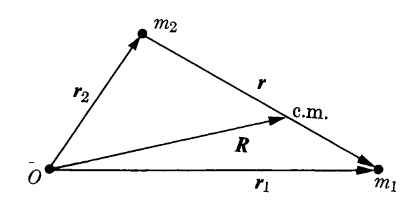
\includegraphics[scale=0.5]{Images/twoBodyProblem.png}
  	\caption{Posición de ambos cuerpos en el espacio, representando su posicion relativa y respecto a un sistema de coordenadas $O$. El vector $\vb{R}$ representa la posición del centro de masa relativa al sistema $O$. Imagen extraída de \cite{b1}, cap $4$.}
  	\label{fig:twoBodyProblem}
\end{figure}

Además, la ecuación de movimiento
\begin{displaymath}
	\mu \ddot{\vb{r}_{21}} = \vb{F}, \quad \quad \mu = \frac{M_1 M_2}{M_1 M_2},
\end{displaymath}

\noindent
al término $\mu$ se le conoce como masa reducida\footnote{De \cite{b2} capítulo $8$, sección $2$}. Para la fuerza gravitacional y una trayectoria circular, la expresión para frecuencia angular del sistema, se tiene
\begin{displaymath}
	\omega ^2 = \frac{G(M_1 + M_2)}{a^3}.
\end{displaymath}
 
\subsubsection{Sistema de Referencia Estrellado}

Para simplificar el análisis del problema, se introduce un sistema en movimiento, en concreto, en rotación. Esto es para eliminar el movimento de los cuerpos más masivos, a este nuevo sistema le llamaremos $O^*$. Este nuevo sistema tendrá su origen en el centro de masa y, a la distancia entre los cuerpos se le llamará $a$. De modo que las posiciónes en $O^*$ están dadas solo en el eje $x^*$ como
\begin{displaymath}
	x_1 = \frac{M_2}{M_1 + M_2}a, \quad x_2 = -\frac{M_1}{M_1 + M_2}a;
\end{displaymath}

\noindent
además, se fija $\vec{\omega} = \omega \vz$ y la masa $m$ solo se mueve en el plano $x^* y^*$. Con todo esto, la ecuación de moviento en el sistema $O^*$
\begin{displaymath}
	m\frac{\text{d}^{*2} r}{\text{d} t^2} = F_1 + F_2 - m\omega \cp (\omega \cp r) - 2m\omega \cp \frac{\text{d}^* r}{\text{d} t}.
\end{displaymath}

\noindent
En la cual las dos fuerzas representadas son las fuerzas de cada una de las masas sobre la masa $m$ orbitando. Expresandolas en componentes
\begin{displaymath}
	F_1 = \frac{GM_1 m}{\qty((x - x_1)^2 + y^2)^{\flatfrac{3}{2}}} (x - x_1,y), \quad \quad F_2 = \frac{GM_2 m}{\qty((x - x_2)^2 + y^2)^{\flatfrac{3}{2}}} (x - x_2,y).
\end{displaymath}


Analizando el resto de términos, se tiene que la fuerza de coriolis es perpendicular a la velocidad, por lo que no ningún trabajo. Para el término de la fuerza centrífuga, es sencillo corroborar que es una fuerza central\footnote{Fuerza radial conservativa.}, lo que implica que tiene una energía potencial asociada. Desarrollando el término de la fuerza centrífuga y encontrando el potencial
\begin{align*}
	- m\omega \cp (\omega \cp r) &= m\omega ^2 \qty(x\mathbb{\vu{x} ^*} + y \mathbb{\vu{y} ^*}) \\
	V_c &= -\frac{1}{2} m\omega ^2 (x^2 + y^2).
\end{align*}

Con el análisis anterior, se concluye que la enería potencial total del sistema es
\begin{displaymath}
	V = -\frac{GM_1 m}{\qty((x - x_1)^2 + y^2)^{\flatfrac{1}{2}}} - \frac{GM_2 m}{\qty((x - x_2)^2 + y^2)^{\flatfrac{1}{2}}} - \frac{1}{2} m\omega ^2 \qty(x^2 + y^2).
\end{displaymath}

\noindent
Por simplicidad no se tomara la enería potencial, sino que el potencial gravitacional del sistema, para que no halla dependencia de una masa arbitraria
\begin{displaymath}
	\mathcal{G} = -\frac{GM_1}{\qty((x - x_1)^2 + y^2)^{\flatfrac{1}{2}}} - \frac{GM_2}{\qty((x - x_2)^2 + y^2)^{\flatfrac{1}{2}}} - \frac{1}{2} \omega ^2 \qty(x^2 + y^2).
\end{displaymath}


\subsection{Puntos de Lagrange}
Para un sistema de dos cuerpos, los puntos de lagrange son las posiciones en donde un objeto/satélite podría estar en reposo respecto al sistema orbital. Estos puntos representan las posiciones en donde la atracción del sistema presenta una rotación sincrónica con la menor masa del sistema. Matemáticamente hablando, son las soluciones de equilibrio al problema de los $3$ cuerpos restringido. Para cualquier sistema de $3$ cuerpos existen $5$ de estos puntos de lagrange, representados por $L_1,L_2,L_3,L_4$ y $L_5$. 












\section{Implementación}
\label{sec:implementacion}

\subsection{Simplificación del Modelo}

Para que la implementación sea más simple, y que el programa/lenguaje que se utilize no gaste recursos trabajando con números de grandes ordenes de magnitud o de ordenes muy pequeños. Se realizará el siguiente cambio de variables $\xi = x/a$ y $\eta = y/a$, con lo que
\begin{displaymath}
	\xi _1 = \frac{x_1}{a}, \quad \quad \xi _2 = \frac{x_2}{a} = \xi _1 - 1,
\end{displaymath}

lo que reduce la posicion de cada masa a un número entre $0$ y $1$. Dado esto, el potencial gravitacional se reescribe a (sustituyendo $M_1$ y $M_2$ despejados de las expresiones de $\xi _1$ y $\xi _2$, esto para tener una expresión más amigables)
\begin{displaymath}
	\mathcal{G} (\xi, \eta) = \frac{G(M_1 + M_2)}{a} \qty[\frac{\xi _2}{\sqrt{(\xi - \xi _1)^2 + \eta ^2}} - \frac{\xi _1}{\sqrt{(\xi - \xi _2)^2 + \eta ^2}} - \frac{1}{2} \qty(\xi ^2 + \eta ^2)],
\end{displaymath}

la implementación se realizó en el sistema $(\xi, \eta)$.


\subsection{Implementación en \textit{Gnuplot}}

El codigo generado, al no ser un algoritmo como tal, no se mostrará el pseudocódigo, pero si se desea ver el codigo utilizado, revisar la sección de anexos \ref{sec:anexos}.

\subsubsection{Sistema Tierra$-$Luna}
Dadas las masas $M_{e} = 5.972\times 10^{24} kg$ y $M_l = 7.329\times 10^{22} kg$, se encuentran las posiciones respectivas respecto al origen del sistema estrellado en coordenadas $(\xi ,\eta)$. De modo que, la superficie potencial y sus curvas de nivel son:

\begin{figure}[H]
\centering
\subfigure[Superficie Potencial]{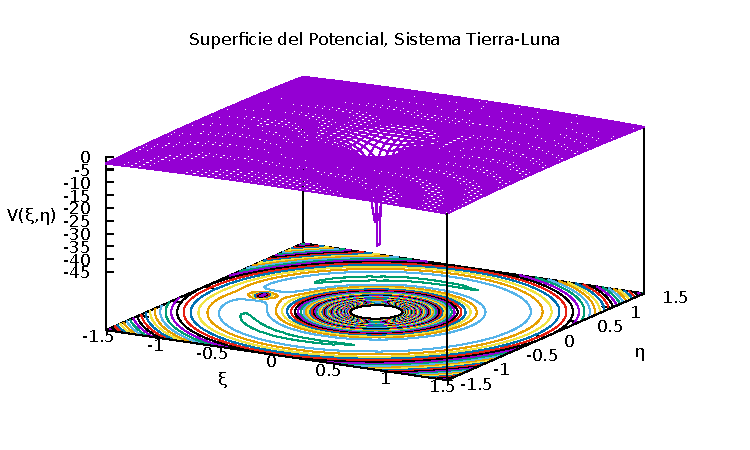
\includegraphics[scale=0.65]{Codigos/surfaceTierraLuna.pdf}}\qquad
\subfigure[Curvas de Nivel]{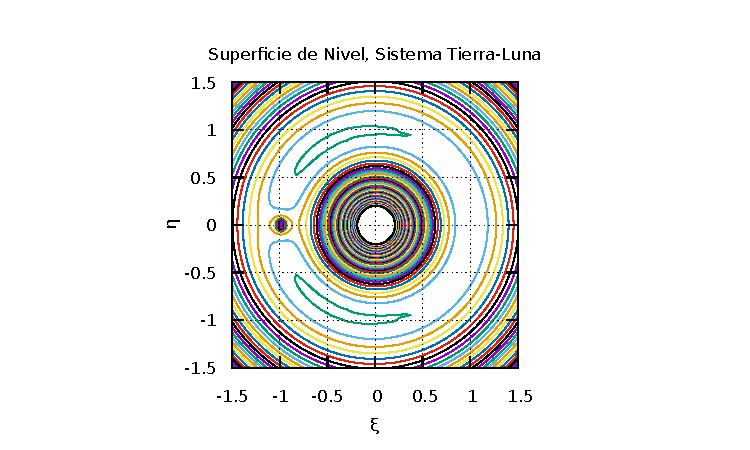
\includegraphics[scale=0.67]{Codigos/contourTierraLuna.pdf}}
\caption{Sistema Tierra$-$Luna: (a) La singularidad en la superficie representa a la tierra. Como se verá más adelante, entre mayor sea la diferencia entre las masas de los cuerpos, menor será la distinción del cuerpo de menor masa. (b) En las curvas de nivel se ven representados, no al nivel que se requiere, los puntos de interes en cierto rango.}
\label{fig: surperficie, cn t-l}
\end{figure}



\begin{multicols}{2}
Para iniciar con algunas aproximaciones de los puntos más evidentes, se toma la coordenada $\eta = 0$. Lo que genera la siguiente curva en dicho plano: 

Lo que facilita los primeros tres puntos de lagrange estan dados en $L_1 \approx (-1.17,0)$, $L_2 \approx (-0.90,0)$ y $L_3 \approx (1,0)$. Estos puntos están representados en el sistema de coordenadas $(\xi ,\eta)$; por lo que, realizando el cambio de sistema correspondiente $x = a\xi$, donde $a$ es la distancia entre ambos cuerpos (para el sistema tierra$-$luna $a = 3.844\times 10^{8} m$), se tiene que $L_1 \approx (-4.497\times 10^{8},0)$, $L_2 \approx (-3.46\times 10^{8},0)$ y $L_3 \approx (3.844\times 10^{8},0)$, todo medido en $m$.
\columnbreak
\begin{figure}[H]
	\centering
	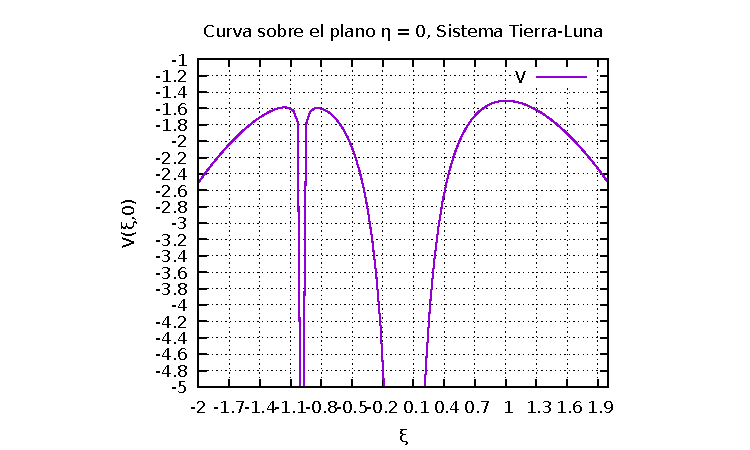
\includegraphics[scale=0.7]{Codigos/planePlotTierraLuna.pdf}
	\caption{Curva sobre el plano $\eta = 0$, bajo un poco de análisis de calculo diferencial, o directamente por las gráficas, se pueden representar los primeros $3$ puntos de Lagrange.}
	\label{fig:planeplot t-l}
\end{figure}
\end{multicols}

Aumentando el número de curvas de nivel se remarca más, el hecho de que los puntos $L_4$ y $L_5$ estan entre las curvas alargadas verdes. Con eso, la parte más gruesa representaría la posición de los puntos, además estan posicionados de modo que genere un triangulo equilátero con las masas como vértices; de modo que, los ultimos dos puntos serían $L_4 \approx (-0.5,0.8)$ y $L_5 \approx (-0.5,-0.8)$, es decir, en términos de coordenadas $(x,y)$: $L_4 \approx (-1.922\times 10^{8},3.075 \times 10^{8})$ y $L_5 \approx (-1.922 \times 10^{8},-3.075 \times 10^{8})$, medido en $m$.





\subsubsection{Sistema Sol$-$Jupiter}
Ya con el procedimiento explicado en el sistema anterior, las gráficas de potenciales y la curva sobre el plano $\eta = 0$, para las masas $M_s = 1.989\times 10 ^{30} kg$ y $M_J = 1.898\times 10 ^{27}$, son: 

\begin{figure}[H]
\centering
\subfigure[Superficie Potencial \label{surface s-j}]{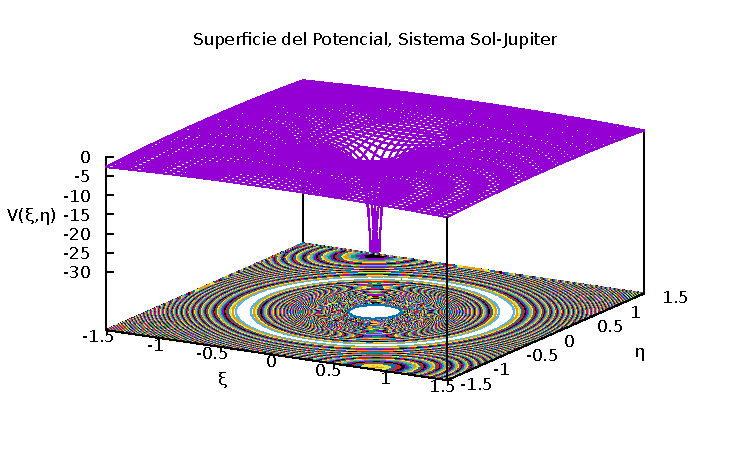
\includegraphics[scale=0.45]{Codigos/surfaceSolJupiter.pdf}}
\subfigure[Curvas de Nivel \label{contour s-j}]{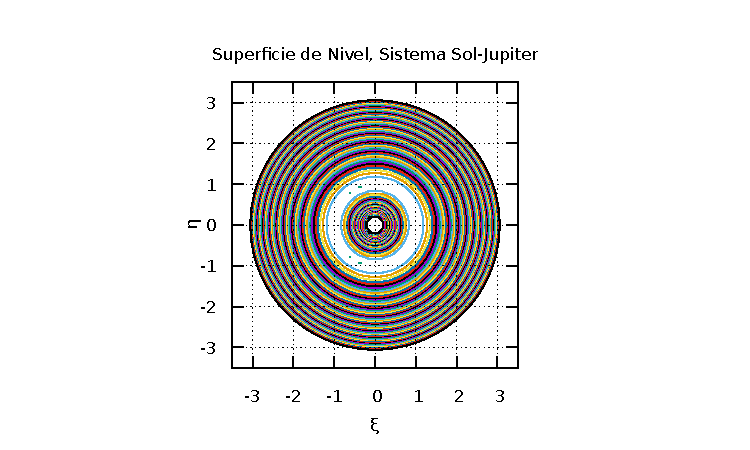
\includegraphics[scale=0.46]{Codigos/contourSolJupiter.pdf}}
\subfigure[Curva en plano \label{plane s-j}]{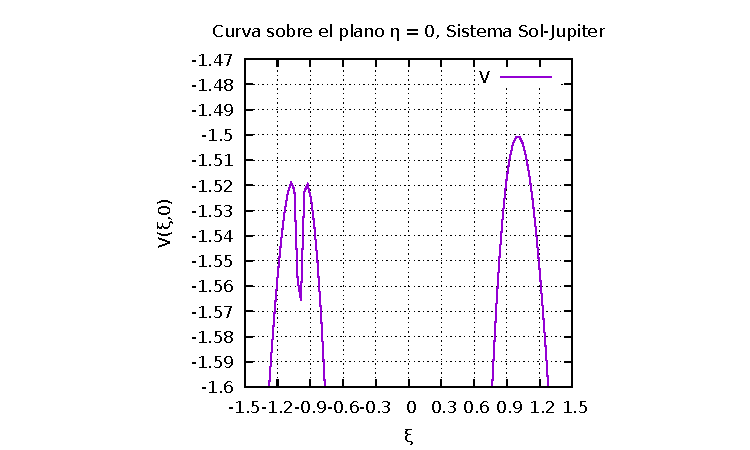
\includegraphics[scale=0.45]{Codigos/planePlotSolJupiter.pdf}}
\caption{Sistema Sol$-$Jupiter: (a) Superficie que representa el potencial gravitacional generado por el sistema. (b) Curvas de nivel, como se mencionó en la figura \ref{fig: surperficie, cn t-l}, entre mayor sea la diferencia entre las masas, menor será la distinción del cuerpo más pequeño. (c) Puntos de Lagrange sobre el plano $\eta = 0$.}
\label{superficie, cn, plane s-j}
\end{figure}

Por lo dicho acerca de la figura \ref{contour s-j}, no se puede calcular la posición de los puntos $L_4$ y $L_5$ directamente; sin embargo, la posición de dichos puntos, esta dada por los dos triangulos equiláteros generados por la distancia entre las masas, lo que nos da los puntos $L_4, L_5 \approx (-0.5,\pm 0.866) \approx (-3.75\times 10^{11},\pm 6.5\times 10^{11})$. Entonces, de la figura \ref{plane s-j} las coordenadas son $L_1 \approx (-1.1,0)$, $L_2 \approx (-0.9,0)$ y $L_3 \approx (1.1,0)$, para $L_4 , L_5 = $. Para encontrar la posición en el plano sistema $(x,y)$, se usa el cambio de coordenadas mostrado en el sistema anterior y la distancia $a = 7.5\times 10^{11}m$: $L_1 \approx (-8.25\times 10 ^{11},0)$, $L_2 \approx (-6.75\times 10 ^{11},0)$ y $L_3 \approx (8.25\times 10 ^{11},0)$, en $m$.



\subsubsection{Sistema Sol$-$Tierra}

Para este sistema, la diferencia de masas es absurdamente grande ($6$ ordenes de magnitud). Las masas de los cuerpos son $M_e = 5.972\times 10^{24} kg$ y $M_s = 1.989\times 10 ^{30} kg$. Por el mismo argumento del sistema anterior, solo se mostrarán los puntos de Lagrange sobre el plano $\eta = 0$.

\begin{figure}[H]
\centering
\subfigure[Superficie Potencial \label{surface s-e}]{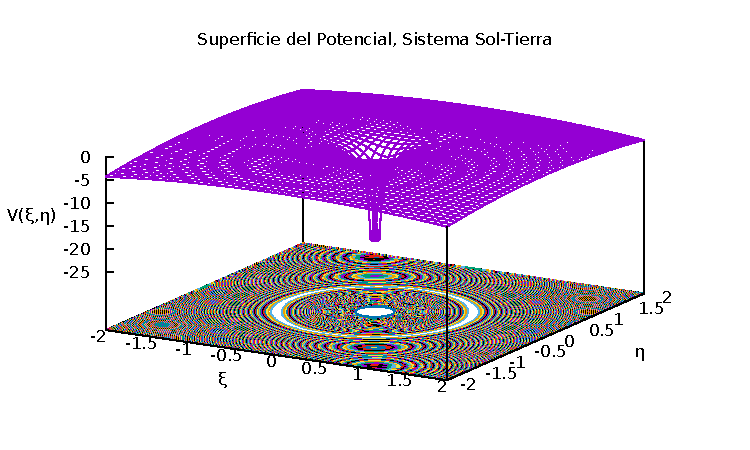
\includegraphics[scale=0.45]{Codigos/surfaceSolTierra.pdf}}
\subfigure[Curvas de Nivel \label{contour s-e}]{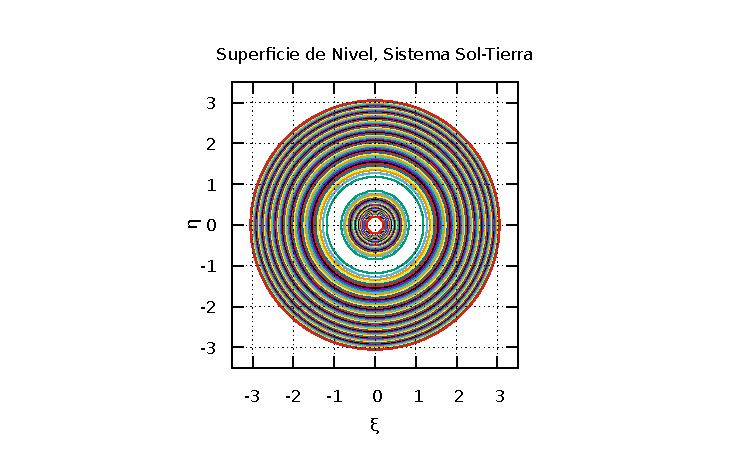
\includegraphics[scale=0.46]{Codigos/contourSolTierra.pdf}}
\subfigure[Curva en plano \label{plane s-e}]{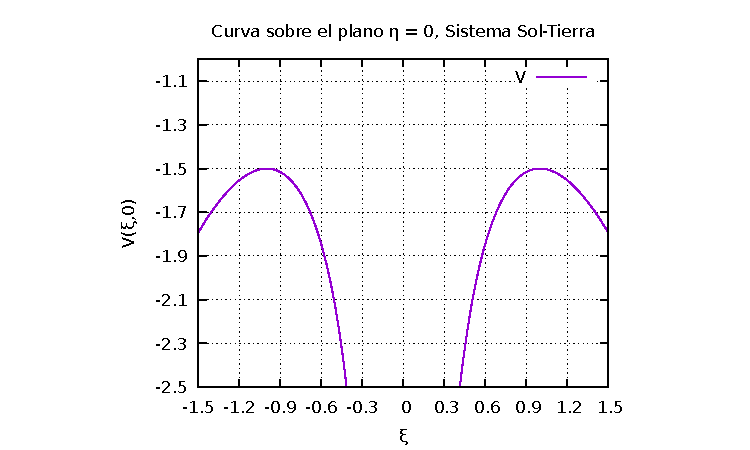
\includegraphics[scale=0.45]{Codigos/planePlotSolTierra.pdf}}
\caption{Sistema Sol$-$Tierra: (a) Superficie potencial para el sistema Sol$-$Tierra, a diferencia de los dos sistemas anteriores, ya no es posible distinguir de ninguna forma la presencia de la tierra en la superficie. (b) Curvas de nivel, al haber $6$ ordenes de magnitud de diferencia entre las masas, no es perceptible la aportación gravitacional de la Tierra comparada con la del sol. (c) Curva sobre el plano $\eta = 0$}
\label{superficie, cn, plane s-j}
\end{figure}

Analizando la gráfica \ref{plane s-e}, es curioso observar que los puntos $L_1$ y $L_2$ son practicamente el mismo (cosa que no es cierta), por lo que $L_1 \approx L_2 \approx (-0.95,0)$ y $L_3 \approx (1,0)$. Convirtiendo al sistema $(x,y)$, se tiene $L_1 \approx L_2 \approx (-1.4212\times 10^{11},0)$ y $L_3 \approx (1.496\times 10^{11},0)$, dado que $a = 1.456\times 10^{11}m$. A pesar de que los ordenes de magnitud son muy diferentes, en base a la hipótesis de que los puntos $L_4$ y $L_5$ forman un triangulo equilátero con la posicion de las masas, y la posición es practicamente $(0,0)$ y $(1,0)$, lo que da $L_4, L_5 \approx (-7.5\times 10^{10},\pm 2.99\times 10^{11}) m$.




\subsection{Implementación en \textit{Mathematica}}

Dadas las implementaciones realizadas en el interprete \textit{Gnuplot}, es claro que se requiere mayor calidad en la imagen para tener una mejor presición al momento de visualizar los datos. \textit{Mathematica} permite realizar esto, de una manera más sencilla y con mejores resultados. Los datos de las masas son exactamente los mismos que la parte anterior, así como las distancias entre objetos de análisis.



\subsubsection{Sistema Tierra$-$Luna}
La gráfica del potencial y sus curvas de nivel son:

\begin{figure}[H]
\centering
\subfigure[Superficie Potencial \label{surface e-l, math}]{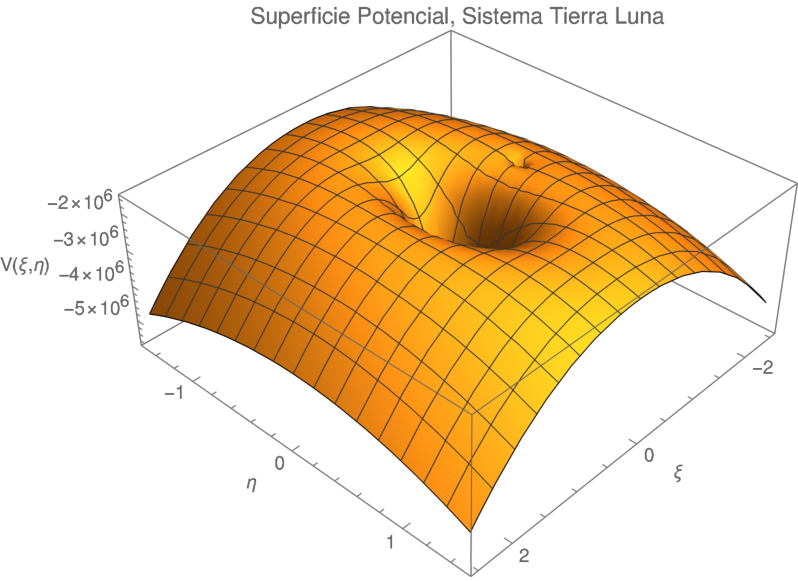
\includegraphics[scale=0.5]{Images/surfaceTierraLuna.pdf}} \qquad \qquad
\subfigure[Curvas de Nivel \label{contour e-l, math}]{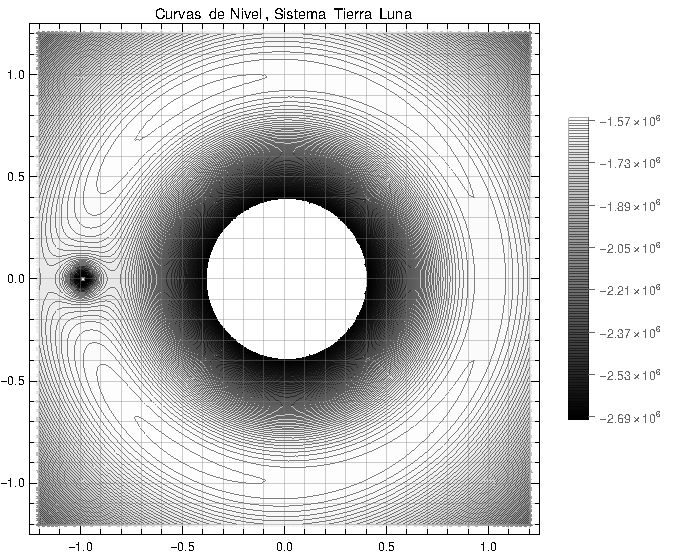
\includegraphics[scale=0.5]{Images/contourTierraLuna.pdf}}
\caption{Sistema Tierra$-$Luna: (a) Superficie potencial, la luna es distinguible como la sigunlaridad pequeña. (b) Curvas de nivel, claramente se muestran los $5$ puntos de interes.}
\label{superficie, cn e-l, math}
\end{figure}

En la figura \ref{contour e-l, math} es claro donde se ubican todos los puntos de interes; por lo que, los puntos de lagrange de una forma más precisa son (puntos de Lagrange representados en ambos sistemas): $L_1 \approx (-1.15,0) \approx (-4.42\times 10^{8} ,0)$, $L_2 \approx (-0.835,0) \approx (-3.21\times 10^{8} ,0)$, $L_3 \approx (1,0) \approx (3.844\times 10^{8} ,0)$, $L_4 \approx (-0.6,0.8) \approx (-2.31\times 10^{8} ,3.075\times 10^{8})$ y $L_5 \approx (-0.6,-0.8) \approx (-2.31\times 10^{8} ,-3.075\times 10^{8})$. \\

Dadas las aproximaciones gráficas, para comparar los datos con una solución directa del problema con bases en el cálculo. Sabiendo que los máximos o mínimos de una función se encuentrar por medio de la primera derivada igualada a cero. Como estamos trabajando con funciones de dos variables se genera un sistema de ecuaciones igualando las primeras derivadas a cero, es decir
\begin{displaymath}
	\left\{\begin{array}{cc}
		\displaystyle\pdv{\mathcal{G}}{\xi} = 0 & \\
		& \\
		\displaystyle\pdv{\mathcal{G}}{\eta} = 0. & 
	\end{array}\right.
\end{displaymath}

El sistema generado no es soluble analíticamente, por lo que se realiza una solución numérica con la función \texttt{NSolve[\{D[G,$\xi$] $== 0$,D[G,$\eta$] $== 0$\},\{$\xi,\eta$\}]}. Lo que nos devuelve un arreglo con los puntos de Lagrange, los cuales son: $L_1 = (-1.1557,0) = (-4.44\times 10^{8},0)$, $L_2 = (-0.83689, 0) = (-3.22\times 10^{8},0)$, $L_3 = (1.005, 0) = (3.863\times 10^{8},0)$, $L_4 = (-0.4878, 0.866) = (-1.875\times 10^{8},3.33\times 10^{8})$ y $L_5 = (-0.4878, -0.866) = (-1.875\times 10^{8},-3.33\times 10^{8})$. \\

Comparando los tres datos recopilados, es claro que, a pesar de la discrepacia que pueda haber (que mayormente puede ser debida al hecho de ser método gráfico), practicamente coinciden, lo que refuerza las validez de las medidas.



\subsubsection{Sistema Sol$-$Jupiter}
Las gráficas representativas del sistema:

\begin{figure}[H]
\centering
\subfigure[Superficie Potencial \label{surface s-j, math}]{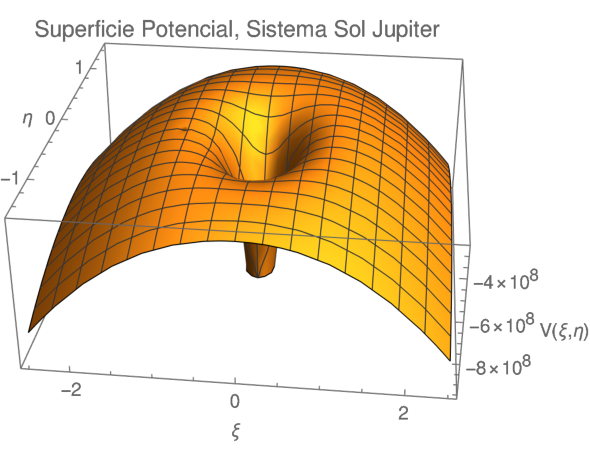
\includegraphics[scale=0.55]{Images/surfaceSolJupiter.pdf}} \qquad \qquad
\subfigure[Curvas de Nivel \label{contour s-j, math}]{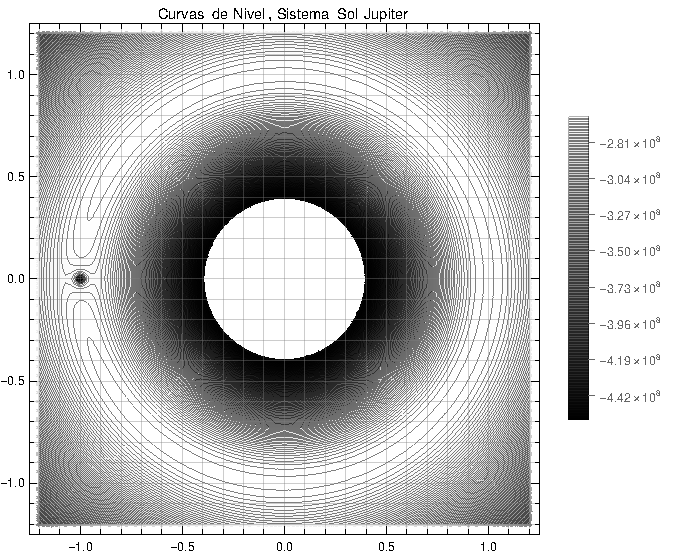
\includegraphics[scale=0.55]{Images/contourSolJupiter.pdf}}
\caption{Sistema Sol$-$Jupiter: (a) Superficie potencial, Jupiter es apenas distinguible. (b) Curvas de nivel, los puntos $4$ y $5$ ya no son tan distinguibles, con la idea de la implementación en gnuplot, se puede conjeturar la posición.}
\label{superficie, cn s-j, math}
\end{figure}

En base a \ref{contour s-j, math}, las posiciones de los puntos de Lagrange, en ambos sistemas, son: $L_1 \approx (-1.06,0) \approx (-7.95\times 10^{11} ,0)$, $L_2 \approx (-0.94,0) \approx (-7.05\times 10^{11} ,0)$, $L_3 \approx (1,0) \approx (7.5\times 10^{11} ,0)$, $L_4 \approx (-0.5,0.85) \approx (-3.75\times 10^{11} ,6.375\times 10^{11})$ y $L_5 \approx (-0.5,-0.85) \approx (-3.75\times 10^{11} ,-6.375\times 10^{11})$, medido en $m$. \\

Realizando el mismo procedimiento que en sistema anterior, se encuentran los siguientes puntos de Lagrange, por medio de métodos numéricos: $L_1 = (-1.0688,0) = (-8.016\times 10^{11} ,0)$, $L_2 = (-0.9324,0) = (-6.993\times 10^{11} ,0)$, $L_3 = (1,0) = (7.5\times 10^{11} ,0)$, $L_4 = (-0.499,0.866) = (-3.7425\times 10^{11} ,6.495\times 10^{11})$ y $L_5 = (-0.499,-0.866) = (-3.7425\times 10^{11} ,-6.495\times 10^{11})$, medido en $m$. 

\newpage

\subsubsection{Sistema Sol$-$Tierra}

Gráficas representativas:

\begin{figure}[H]
\centering
\subfigure[Superficie Potencial \label{surface s-e, math}]{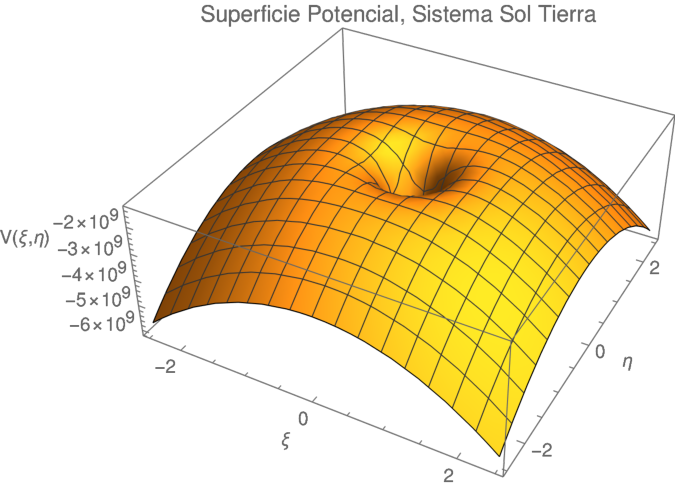
\includegraphics[scale=0.4]{Images/surfaceSolTierra.pdf}} \qquad
\subfigure[Curvas de Nivel \label{contour s-e, math}]{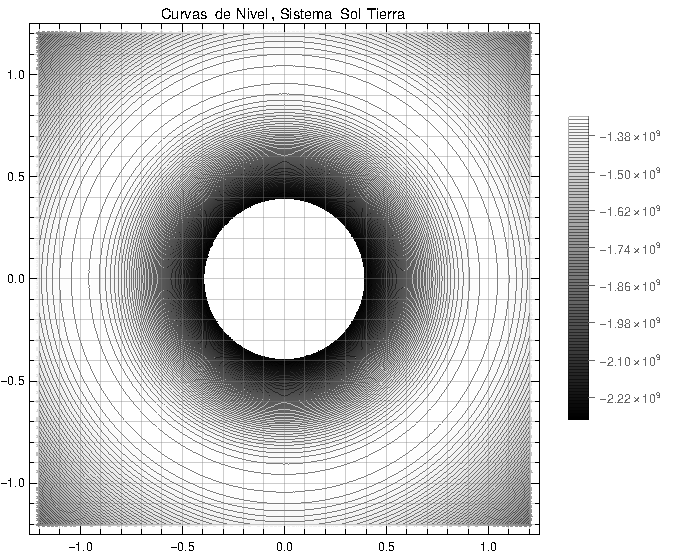
\includegraphics[scale=0.4]{Images/contourSolTierra.pdf}} \qquad
\subfigure[Curva en plano \label{contour s-e, math}]{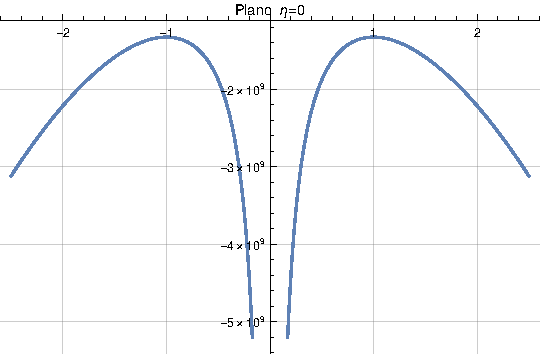
\includegraphics[scale=0.5]{Images/planePlotSolTierra.pdf}}
\caption{Sistema Sol$-$Tierra: (a) Superficie potencial, la Tierra no es distinguible, la diferencia en ordenes de magnitud. (b) Curvas de nivel, los puntos no son distinguibles. (c) Así como en la implementación en \textit{Gnuplot}, no es perceptible la contribución gravitacional de la tierra, los puntos $L_1$ y $L_2$ practicamente en el mismo punto (gráficamente hablado, es claro que físicamente no es cierto).}
\label{superficie, cn s-e, math}
\end{figure}

Gráficamente, de \ref{contour s-e, math}, solo es posible encontrar los primeros $3$ puntos de Lagrange: $L_1 \approx L_2 \approx (-1,0) \approx (-1.5\times 10^{11},0)$ y $L_3 \approx (1,0) \approx (1.5\times 10^{11},0)$. Para los puntos $L_4$ y $L_5$ se utiliza la idea de lo realizado con la implementación en \textit{Gnuplot}, $L_4,L_5 \approx (-7.5\times 10^{10},\pm 2.99\times 10^{11})$ \\

Utilizando métodos numéricos, los puntos de Lagrange para el sistema son: $L_1 = (-1.01, 0) = (-1.515\times 10^{11} ,0)$, $L_2 = (-0.99, 0) = (-1.485\times 10^{11} ,0)$, $L_3 = (1,0) = (1.5\times 10^{11} ,0)$, $L_4 = (-0.499997, 0.866) = (-7.49996\times 10^{10} ,1.299\times 10^{11})$ y $L_5 = (-0.499997,-0.866) = (-7.49996\times 10^{10} ,-1.299\times 10^{11})$, medido en $m$.





\section{Resultados}
\label{sec:resultados}

Las tablas de resultados para cada los $5$ puntos de Lagrange de cada sistema, encontrados de las $3$ formas anteriormente planteadas. Las posiciones estarán dadas en el sistema $(x,y)$.

\subsection{Sistema Tierra$-$Luna}

\begin{table}[H]
\centering
	\caption{Puntos de Lagrange en coordenadas $(x,y)$, sistema Tierra$-$Luna.}
	\begin{tabular}{||c||c|c|c|c||}
		\hline
		\hline
		Implementación & $L_1$ & $L_2$ & $L_3$ & $L_4 ,L_5$ \\
		\hline
		\hline
		Gnuplot & $(-4.497\times 10^{8} ,0)$ & $(-3.46\times 10^{8} ,0)$ & $(3.84\times 10^8 ,0)$ & $(-1.92\times 10^8 ,\pm 3.075\times 10^8)$ \\
		\hline
		Mathematica & $(-4.42\times 10^{8} ,0)$ & $(-3.21\times 10^{8} ,0)$ & $(3.84\times 10^{8} ,0)$ & $(-2.31\times 10^{8} ,\pm 3.075\times 10^{8})$ \\
		\hline
		Numérica & $(-4.44\times 10^{8},0)$ & $(-3.22\times 10^{8},0)$ & $(3.86\times 10^{8},0)$ & $(-1.88\times 10^{8},\pm 3.33\times 10^{8})$ \\
		\hline
		\hline
	\end{tabular}
	\label{tab:t-l}
\end{table}





\subsection{Sistema Sol$-$Jupiter}

\begin{table}[H]
\centering
	\caption{Puntos de Lagrange en coordenadas $(x,y)$, sistema Sol$-$Jupiter.}
	\begin{tabular}{||c||c|c|c|c||}
		\hline
		\hline
		Implementación & $L_1$ & $L_2$ & $L_3$ & $L_4 ,L_5$ \\
		\hline
		\hline1
		Gnuplot & $(-8.25\times 10 ^{11},0)$ & $(-6.75\times 10 ^{11},0)$ & $(8.25\times 10 ^{11},0)$ & $(-3.75\times 10^{11},\pm 6.5\times 10^{11})$ \\
		\hline
		Mathematica & $(-7.95\times 10^{11} ,0)$ & $(-6.99\times 10^{11} ,0)$ & $(7.5\times 10^{11} ,0)$ & $(-3.74\times 10^{11} ,\pm 6.495\times 10^{11})$ \\
		\hline
		Numérica & $(-8.02\times 10^{11} ,0)$ & $(-6.99\times 10^{11} ,0)$ & $(7.5\times 10^{11} ,0)$ & $(-3.74\times 10^{11} ,\pm 6.495\times 10^{11})$ \\
		\hline
		\hline
	\end{tabular}
	\label{tab:t-l}
\end{table}


\subsection{Sistema Sol$-$Tierra}

\begin{table}[H]
\centering
	\caption{Puntos de Lagrange en coordenadas $(x,y)$, sistema Sol$-$Tierra.}
	\begin{tabular}{||c||c|c|c|c||}
		\hline
		\hline
		Implementación & $L_1$ & $L_2$ & $L_3$ & $L_4 ,L_5$ \\
		\hline
		\hline
		Gnuplot & $(-1.42\times 10^{11},0)$ & $(-1.42\times 10^{11},0)$ & $(1.496\times 10^{11},0)$ & $(-7.5\times 10^{10},\pm 2.99\times 10^{11})$ \\
		\hline
		Mathematica & $(-1.5\times 10^{11},0)$ & $(-1.5\times 10^{11},0)$ & $(1.5\times 10^{11},0))$ & $(-7.5\times 10^{10},\pm 2.99\times 10^{11})$ \\
		\hline
		Numérica & $(-1.52\times 10^{11} ,0)$ & $(-1.48\times 10^{11} ,0)$ & $(1.5\times 10^{11} ,0)$ & $(-7.5\times 10^{10} ,\pm 1.3\times 10^{11})$ \\
		\hline
		\hline
	\end{tabular}
	\label{tab:t-l}
\end{table}

\subsection{Representación Gráfica}

\begin{figure}[H]
\centering
\subfigure[Sistema Tierra$-$Luna \label{lag t-lj}]{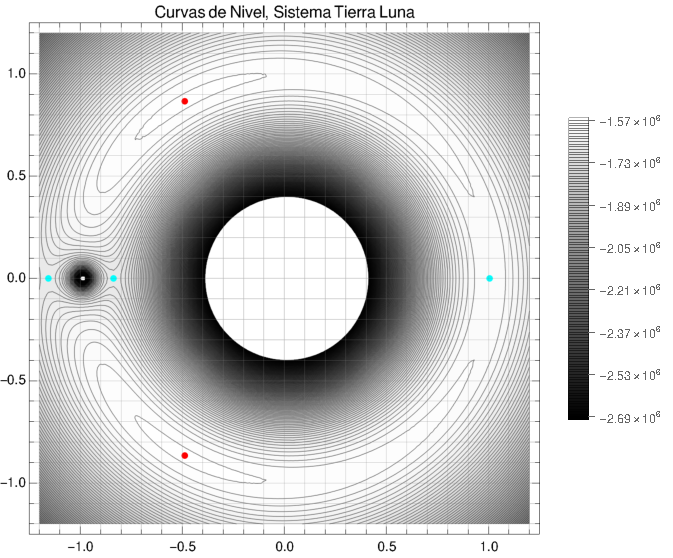
\includegraphics[scale=0.5]{Images/contourTierraLunaLagrange.pdf}}
\subfigure[Sistema Sol$-$Jupiter \label{lag s-j}]{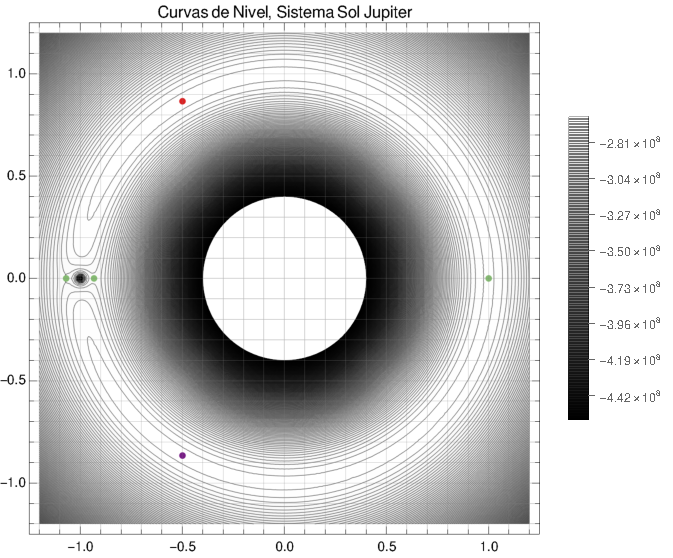
\includegraphics[scale=0.5]{Images/contourSolJupiterLagrange.pdf}}
\subfigure[Sistema Sol$-$Tierra \label{lag s-t}]{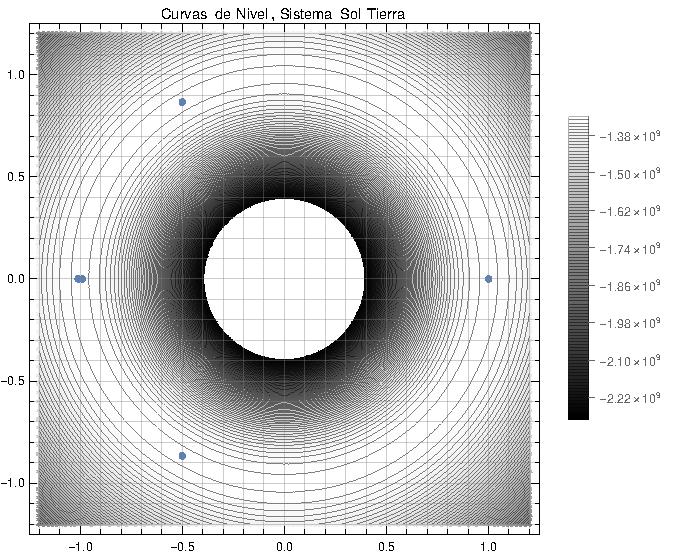
\includegraphics[scale=0.5]{Images/contourSolTierraLagrange.pdf}}
\caption{Cada sistema planetario representado por sus curvas de nivel y los puntos de Lagrange encontrados.}
\label{superficie, cn, plane s-j}
\end{figure}



\section{Discución de Resultados}
\label{sec:discucion}

Los resultados obtenidos con cada uno de los métodos y lenguajes utilizados se sustentan entre sí. El método gráfico, el cual es el más impreciso, también dió valores acordes a lo esperado por medio de las soluciones numéricas. Sin embargo, para sistemas con mayor diferencia en ordenes de magnitud entre las masas, el método gráfico dejaría de ser viable para el calculo de puntos de lagrange, puesto que las imagenes no tienen una resolución ni presición infinita. \\

Además, las soluciones numéricas devuelven más puntos de los que se espera, esto es normal puesto que los puntos extras difieren de manera insignificante ($\approx 10^{-6}$, revisar notebook en el repositorio\footnote{Repositorio: \href{https://github.com/DSarceno/Semestre5/tree/main/Mecanica2/Proyecto/Informe}{\textit{GitHub}}}). Asimismo, los métodos numericos pueden ser suceptibles a pequeñas variaciones, es decir, al tratarse de una región en la que se encuentra el punto máximo, puntos muy cercanos a este, puede que el mismo método también los considere máximos. Como se mencionó, la diferencia es insignificante, por lo que el método numérico devuelve $5$ puntos de Lagrange.


\section{Conclusiones}
\label{sec:conclusiones}

Los resultados obtenidos, para el modelo explicado en la sección \ref{sec:Puntos de Lagrange} y al inicio de la sección \ref{sec:implementacion}, son válidos y sustentables bajo métodos precisos. Sin embargo, al compararlos con los datos reales proporcionados en Wikipedia, extraidos de páginas oficiales de la NASA, algunos de los puntos tienen una discrepacia significativa, esto es debido a las restricciones del modelo, es decir, las orbitas circulares; además, de las no consideraciones de los efectos gravitacionales externos al sistema. A pesar de ello, las aproximaciones encontradas en el trabajo son válidas y muy buenas en relación al modelo resuelto y las herramientas utilizadas.


\section{Anexos}
\label{sec:anexos}

\subsection{Códigos \textit{Gnuplot}}
Los códigos creados para el análisis bajo el lenguaje de \textit{Gnuplot} son en principio iguales para cada sistema, asi que solo se mostrarán para cada tipo de gráfica un único código\footnote{Cada código se ejecuta en terminal desde la carpeta en la que se encuentre el archivo con la siguiente línea: \\
\texttt{gnuplot <filename.gp>}}. \vspace*{0.2cm}

\begin{multicols}{2}
\subsubsection{Superficie de Potencial}
\begin{lstlisting}
# PROGRAM
# terminal
set terminal pdf
set output 'surfaceSolJupiter.pdf'

# divisiones en la superficies para una mejor vision
set isosamples 50

# labels
set title 'Superficie del Potencial, Sistema Sol-Jupiter'
set xlabel 'xi'
set ylabel 'eta'
set zlabel 'V(xi,eta)'

# superficies de nivel
set size ratio -1
set nokey
set contours
set cntrparam levels incremental -5,0.005,0


## plot
# ranges
set xrange [-1.5:1.5]
set yrange [-1.5:1.5]

# constantes
xi1 = M2/(M2 + M1)
xi2 = xi1 - 1

splot ( xi2/sqrt((x - xi1)**2 + y**2) - xi1/sqrt((x - xi2)**2 + y**2) - 0.5*(x**2 + y**2) ) t 'V'

# END PROGRAM
\end{lstlisting}	

\subsubsection{Curvas de Nivel}
\begin{lstlisting}
# PROGRAM
# terminal
set terminal pdf
set output 'contourSolTierra.pdf'

# divisiones en la superficies para una mejor vision
set isosamples 50

# labels
set title 'Superficie de Nivel, Sistema Sol-Tierra'
set xlabel 'xi'
set ylabel 'eta'

# superficies de nivel
set size ratio -1
set grid
set view map
set nokey
unset surface
set contour base
set cntrparam levels incremental -5,0.05,0


## plot
# ranges
set xrange [-3.5:3.5]
set yrange [-3.5:3.5]

# constantes
xi1 = M2/(M2 + M1)
xi2 = xi1 - 1

splot ( xi2/sqrt((x - xi1)**2 + y**2) - xi1/sqrt((x - xi2)**2 + y**2) - 0.5*(x**2 + y**2) ) t 'V'

# END PROGRAM
\end{lstlisting}	

\subsubsection{Plano $\eta = 0$}

\begin{lstlisting}
# PROGRAM
# Idioma
set encoding utf8
# terminal
set terminal pdf
set output 'planePlotSolTierra.pdf'

# labels
set title 'Curva sobre el plano eta = 0, Sistema Sol-Tierra'
set xlabel 'xi'
set ylabel 'V(xi,0)'

# superficies de nivel
set size ratio 0.8
set grid
#set nokey

## plot
# ranges
set xrange [-1.5:1.5]
set xtics -1.5,0.3,1.5
set yrange [-2.5:-1]
set ytics -2.5,0.2,-1

# constantes
xi1 = M2/(M2 + M1)
xi2 = xi1 - 1
y = 0

plot ( xi2/sqrt((x - xi1)**2 + y**2) - xi1/sqrt((x - xi2)**2 + y**2) - 0.5*(x**2 + y**2) ) t 'V'


# END PROGRAM
\end{lstlisting}
\end{multicols}



\subsection{Código \textit{Mathematica}}
La implementación en el lenguaje de \textit{Mathematica} fue realizada en un Notebook, por estética del informe no se colocaron imagenes del mismo; sin embargo, los códigos utilzados y el notebook de \textit{Mathematica} estan disponibles en un repositorio de \textit{GitHub}, revisar pie de página de \ref{sec:discucion}.

%\section*{Agradecimientos}
%\label{sec:agradecimientos}


% References
\nocite{*}
\bibliographystyle{IEEEannot}%
\bibliography{references}%

\begin{thebibliography}{00}
\bibitem{b1} R. Symon, \textit{Mechanics} 3a. Ed. Addison$-$Wesley Publishing Company, 1971
\bibitem{b2} R. Taylor, \textit{Classical Mechanics}, Edwards Brothers, Inc. 2005.
\end{thebibliography}

\end{document}




%%% Local Variables:
%%% mode: latex
%%% TeX-master: t
%%% End:
